\documentclass[11pt]{beamer}
\usetheme{Madrid}
\usefonttheme{serif}

\usepackage[utf8]{inputenc}
\usepackage[english]{babel}
\usepackage[T1]{fontenc}

% Korean language support
\usepackage{kotex}

\usepackage{amsmath}
\usepackage{amsfonts}
\usepackage{amssymb}
\usepackage{graphicx}
\usepackage{caption}
\usepackage{listings}
\usepackage{xcolor}

\DeclareMathOperator{\sen}{sen}
\DeclareMathOperator{\tg}{tg}

\setbeamertemplate{caption}[numbered]

% Python syntax highlighting settings
\lstdefinestyle{pythonstyle}{
    language=Python,
    basicstyle=\tiny\ttfamily,
    keywordstyle=\color{blue}\bfseries,
    commentstyle=\color{gray}\itshape,
    stringstyle=\color{red},
    numberstyle=\tiny\color{gray},
    showstringspaces=false,
    breaklines=true,
    frame=none,
    numbers=left,
    numbersep=5pt,
    xleftmargin=10pt,
    backgroundcolor=\color{white}
}

\author[Ngseo Kim]{Eungseo(Ngseo) Kim}
\title[MegaBlocks]{Paper Presentation: \\ MegaBlocks: Efficient Sparse Training with Mixture-of-Experts}
\newcommand{\email}{juniormoo@snu.ac.kr}
\setbeamertemplate{navigation symbols}{} 
\institute[]{Seoul National University, Biointelligence Lab} 
\date{\today} 

\bibliographystyle{apalike}



\begin{document}

\begin{frame}
\titlepage
\end{frame}

\begin{frame}{Original Paper Information}
    \begin{block}{Original Authors}
    Trevor Gale\textsuperscript{1}, Deepak Narayanan\textsuperscript{2}, Cliff Young\textsuperscript{3}, Matei Zaharia\textsuperscript{1}
    \end{block}
    
    \begin{block}{Publication}
    MLSys 2023 - Proceedings of Machine Learning and Systems
    \end{block}
    
    \begin{block}{Affiliations}
    \textsuperscript{1} Stanford University, Stanford, California, USA \\
    \textsuperscript{2} Microsoft Research, Redmond, Washington, USA \\
    \textsuperscript{3} Google Research, Mountain View, California, USA
    \end{block}
    
\end{frame}

\begin{frame}{Table of Contents}
\tableofcontents 
\end{frame}

\section{TL;DR}
\begin{frame}{1. TL;DR}
    \begin{block}{The Problem}
    \begin{itemize}
        \item Sparsity enables efficient scaling through conditional computation
        \item MoE leverages sparsity by routing tokens to specific experts
        \item Dynamic routing leads to uneven token distribution across experts
        \item Existing approach: Drop excess tokens, pad insufficient experts
    \end{itemize}
    \end{block}
    
    \begin{block}{MegaBlocks Solution}
    \begin{itemize}
        \item Never drop tokens!
        \item Adapt block-sparse operations
        \item No performance loss, significant Expert Parallelism speedup
    \end{itemize}
    \end{block}
\end{frame}

\section{Key Concepts}
\begin{frame}{2. Key Concepts Overview}
    \begin{block}{Key Concepts to be Covered}
    \begin{itemize}
        \item \textbf{Sparsity}: A concept that activates only necessary components through conditional computation for computational efficiency
        \item \textbf{MoE (Mixture-of-Experts)}: An architecture that combines multiple expert models to scale model capacity efficiently
        \item \textbf{Dynamic Routing}: A mechanism that dynamically assigns each token to appropriate experts
        \item \textbf{Expert Parallelism}: A technique that distributes multiple experts across different devices or processors for efficient parallel computation
    \end{itemize}
    \end{block}
    
\end{frame}

\begin{frame}{2. What is Sparsity?}
    \begin{block}{Conditional Computation}
    Sparsity uses the idea of \textbf{conditional computation}. While in dense models all parameters are used for all inputs, sparsity allows us to only run some parts of the whole system.
    \end{block}
    
    \begin{block}{Scaling Without Computation Overhead}
    Shazeer's work showed that conditional computation allows scaling model size without increasing computation proportionally—thousands of experts can be used in each MoE layer.
    \end{block}
    
    \begin{alertblock}{Challenges}
    \begin{itemize}
        \item \textbf{Uneven batch sizes}: If 10 tokens are batched, 5 might go to one expert and 5 to different experts
        \item \textbf{Underutilization}: This leads to uneven batch sizes and inefficient hardware usage
    \end{itemize}
    \end{alertblock}
\end{frame}

\begin{frame}{2. What is Mixture-of-Experts (MoE)?}
    \begin{block}{Definition}
    MoE is an architecture that combines multiple expert models to achieve high capacity efficiently by routing each input to a small subset of experts.
    MoE leverages sparsity by routing tokens to specific experts, enabling conditional computation without activating all parameters.
    \end{block}
    
    \begin{block}{Key Components}
    \begin{itemize}
        \item \textbf{M experts}: neural networks specializing in different sub-problems
        \item \textbf{Router}: decides which experts to consult for each input
        \item \textbf{Gating network}: computes mixture weights for experts; typically linear
    \end{itemize}
    \end{block}
\end{frame}

\begin{frame}{2. MoE Architecture Details}
    \begin{columns}[T]
        \column{0.5\textwidth}
        \raggedright
        \begin{block}{Mathematical Formulation}
        \footnotesize
        For each token $x$ (or batch $X$), MoE routing works as follows \cite{shazeer2017outrageously, fedus2022switch}:
        \begin{itemize}
            \footnotesize
            \item Router computes logits: $z_m = x^T \theta^{(m)}$ for each expert $m \in [M]$, where $\theta^{(m)} \in \mathbb{R}^d$ is the router parameter for expert $m$
            \item Gate probabilities: $p = \text{softmax}(z)$
            \item Top-k selection: choose $k$ experts with highest probabilities
            \item Expert networks $\{\phi_m\}_{m=1}^M$ (typically FFNs) process routed tokens
            \item Output: weighted combination of selected experts
        \end{itemize}
        \end{block}
        
        \column{0.45\textwidth}
        \raggedright
        \begin{center}
        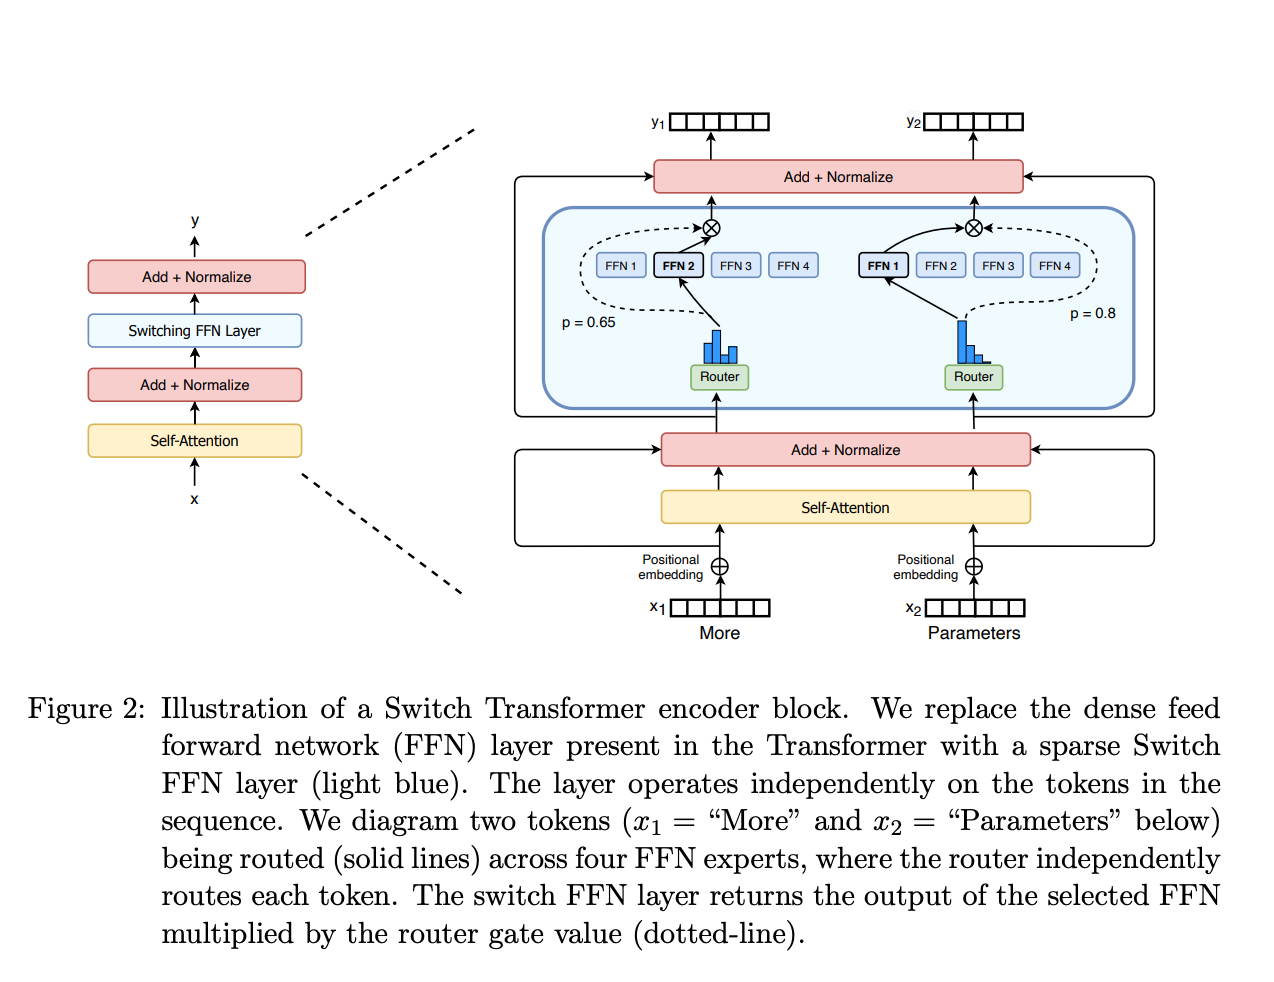
\includegraphics[width=0.85\textwidth]{images/switch_transformer_figure_2.png}
        
        \tiny Figure 1: Switch Transformer architecture.
        \end{center}
    \end{columns}
\end{frame}

\begin{frame}{2. MoE Architecture in MegaBlocks}
    \begin{center}
    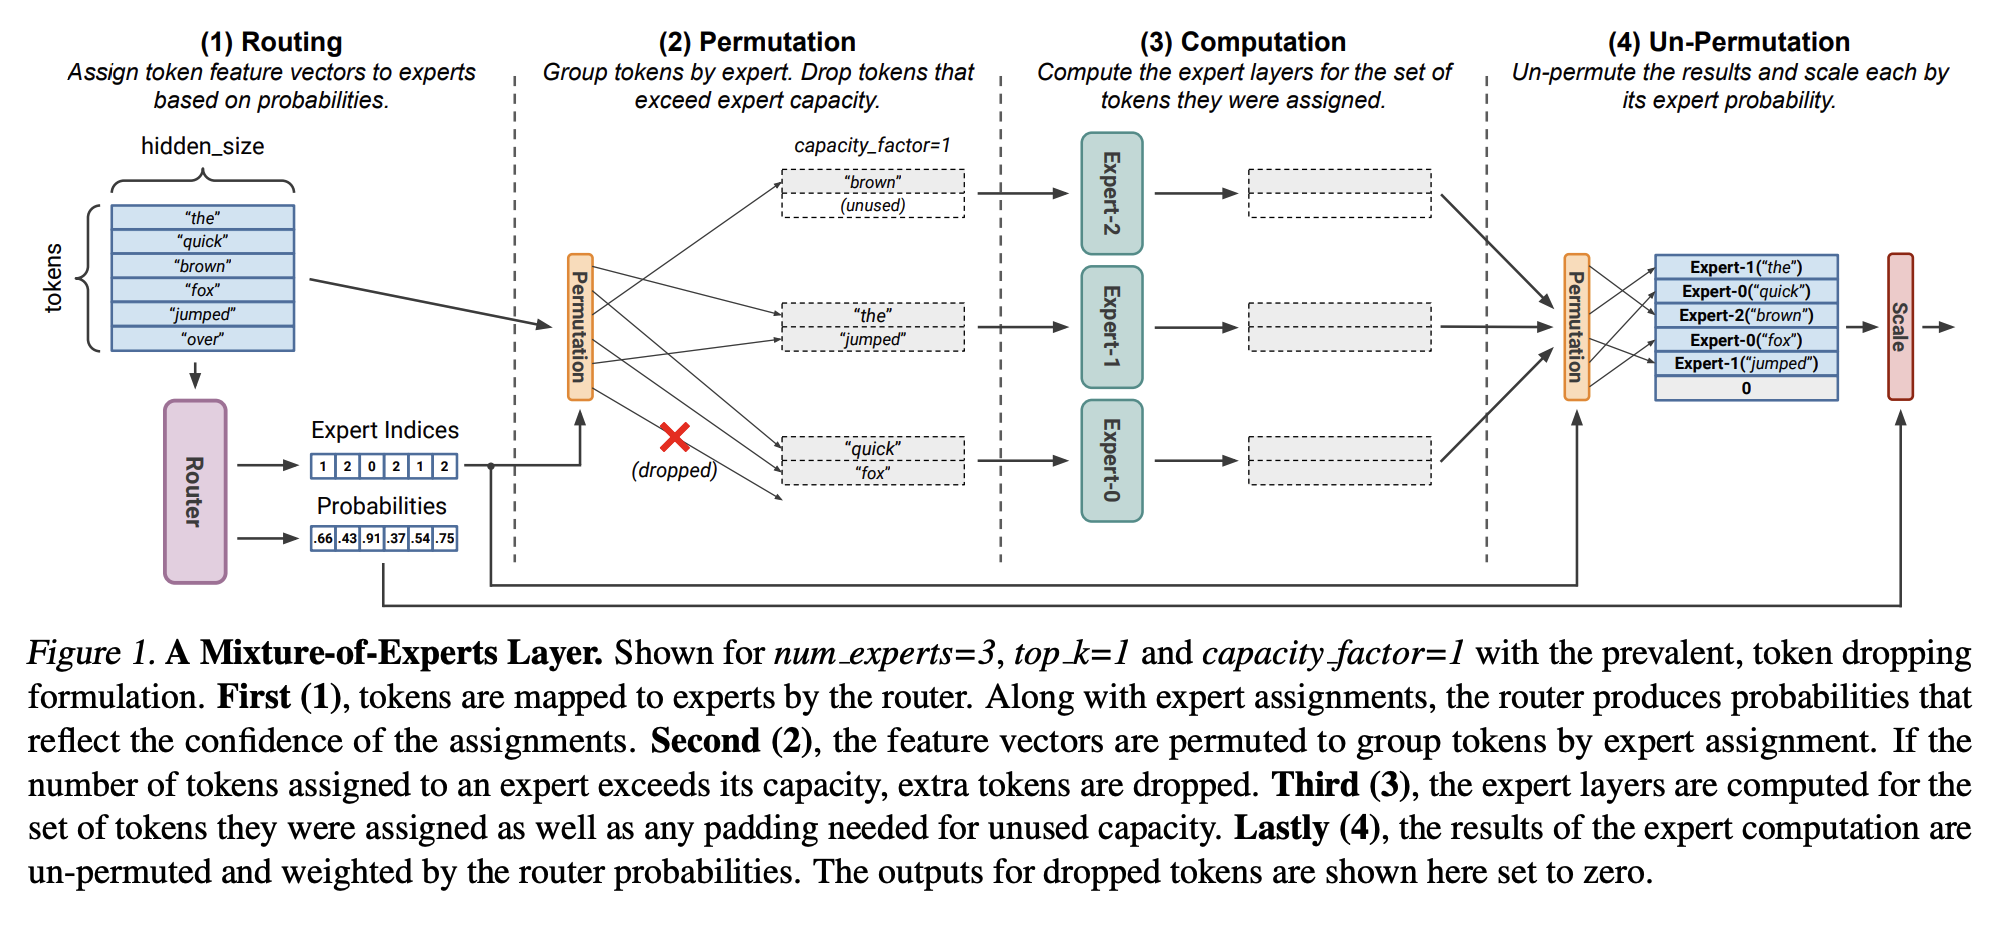
\includegraphics[width=0.95\textwidth]{images/megablocks_moe.png}
    
    \tiny Figure 2: MoE architecture introduced by MegaBlocks.
    \end{center}
\end{frame}

\begin{frame}{2. So Why Dynamic?}
    \begin{block}{What is Dynamic Routing?}
    \footnotesize
    Dynamic routing is a mechanism where the set of selected experts depends on the input. 
    Different inputs are routed to different subsets of experts based on their characteristics.
    \end{block}
    
    \begin{block}{Key Insight}
    \footnotesize
    When input $x$ changes, the set of experts selected also changes:
    \begin{itemize}
        \footnotesize
        \item Different tokens $x_i$ and $x_j$ may be routed to completely different expert subsets
        \item This enables \textbf{input-adaptive computation}: experts specialize in different patterns
        \item Some experts may handle syntax, others semantics—depending on the token
    \end{itemize}
    \end{block}
    
\end{frame}

\begin{frame}{2. Expert Parallelism}
    \begin{center}
    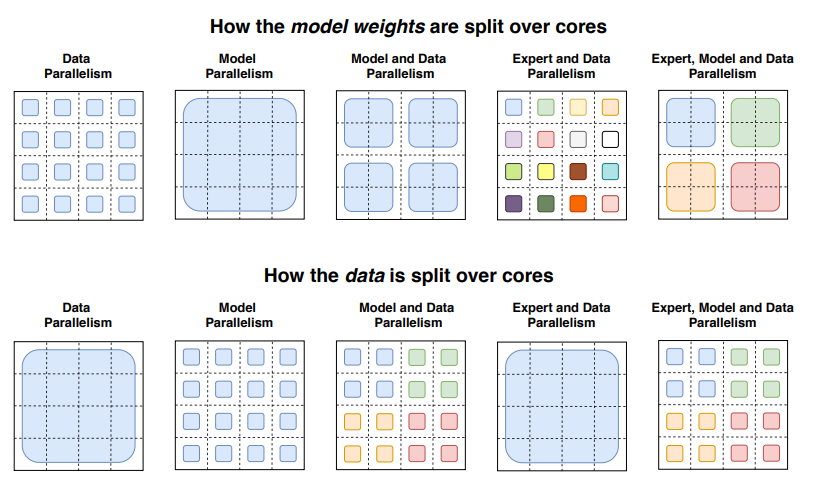
\includegraphics[width=0.75\textwidth]{images/expert_parellelism.png}
    
    \tiny Figure: Expert parallelism architecture \cite{fedus2022switch}.
    \end{center}
    
\end{frame}

\section{Prior Work}
\begin{frame}[shrink]{3. Prior MoE Transformer Training}
    \begin{columns}[T]
        \column{0.55\textwidth}
        \raggedright
        \begin{block}{Fixed Expert Capacity Constraint}
        \scriptsize
        Prior work defines \textbf{fixed expert capacity} \cite{fedus2022switch}:
        \begin{itemize}
            \scriptsize
            \item \textbf{Token dropping}: Excess tokens dropped
            \item \textbf{Padding}: Insufficient experts padded
            \item Static buffer allocation $\rightarrow$ inefficiency
        \end{itemize}
        \end{block}
        
        \vspace{-0.2cm}
        
        \begin{block}{Expert Capacity Formula}
        \scriptsize
        \[
        \text{Expert Capacity} = \frac{\text{num tokens}}{\text{num experts}} \times \text{capacity factor}
        \]
        \vspace{-0.2cm}
        \begin{itemize}
            \scriptsize
            \item Capacity factor: multiplier on uniform distribution
            \item Tradeoff: computation vs. quality
            \item Higher factor $\rightarrow$ less dropping, more padding
        \end{itemize}
        \end{block}
        
        \column{0.4\textwidth}
        \raggedright
        \begin{center}
        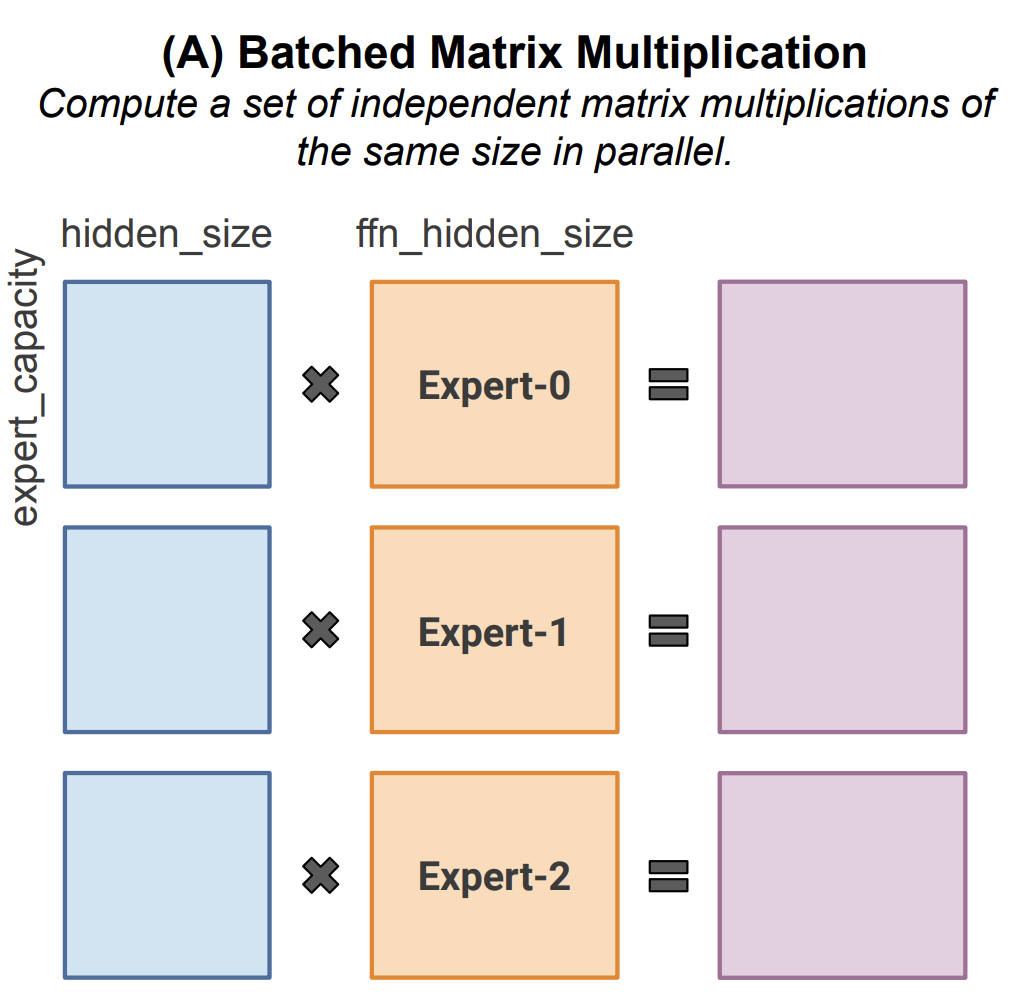
\includegraphics[width=0.75\textwidth]{images/3-a.png}
        
        \tiny Figure: Expert capacity in Switch Transformer.
        \end{center}
    \end{columns}
\end{frame}

\begin{frame}{3. Expert Capacity Factor}
    \begin{columns}[T]
        \column{0.5\textwidth}
        \raggedright
        \begin{block}{Impact of Token Dropping}
        \footnotesize
        Token dropping significantly impacts model quality:
        \begin{itemize}
            \footnotesize
            \item Capacity factor = 1: 0.15 validation loss reduction
            \item Avoiding token dropping: 0.26 reduction (\textbf{1.73× larger})
            \item Higher capacity enables better performance than dense models
        \end{itemize}
        \end{block}
        
        \column{0.45\textwidth}
        \raggedright
        \begin{center}
        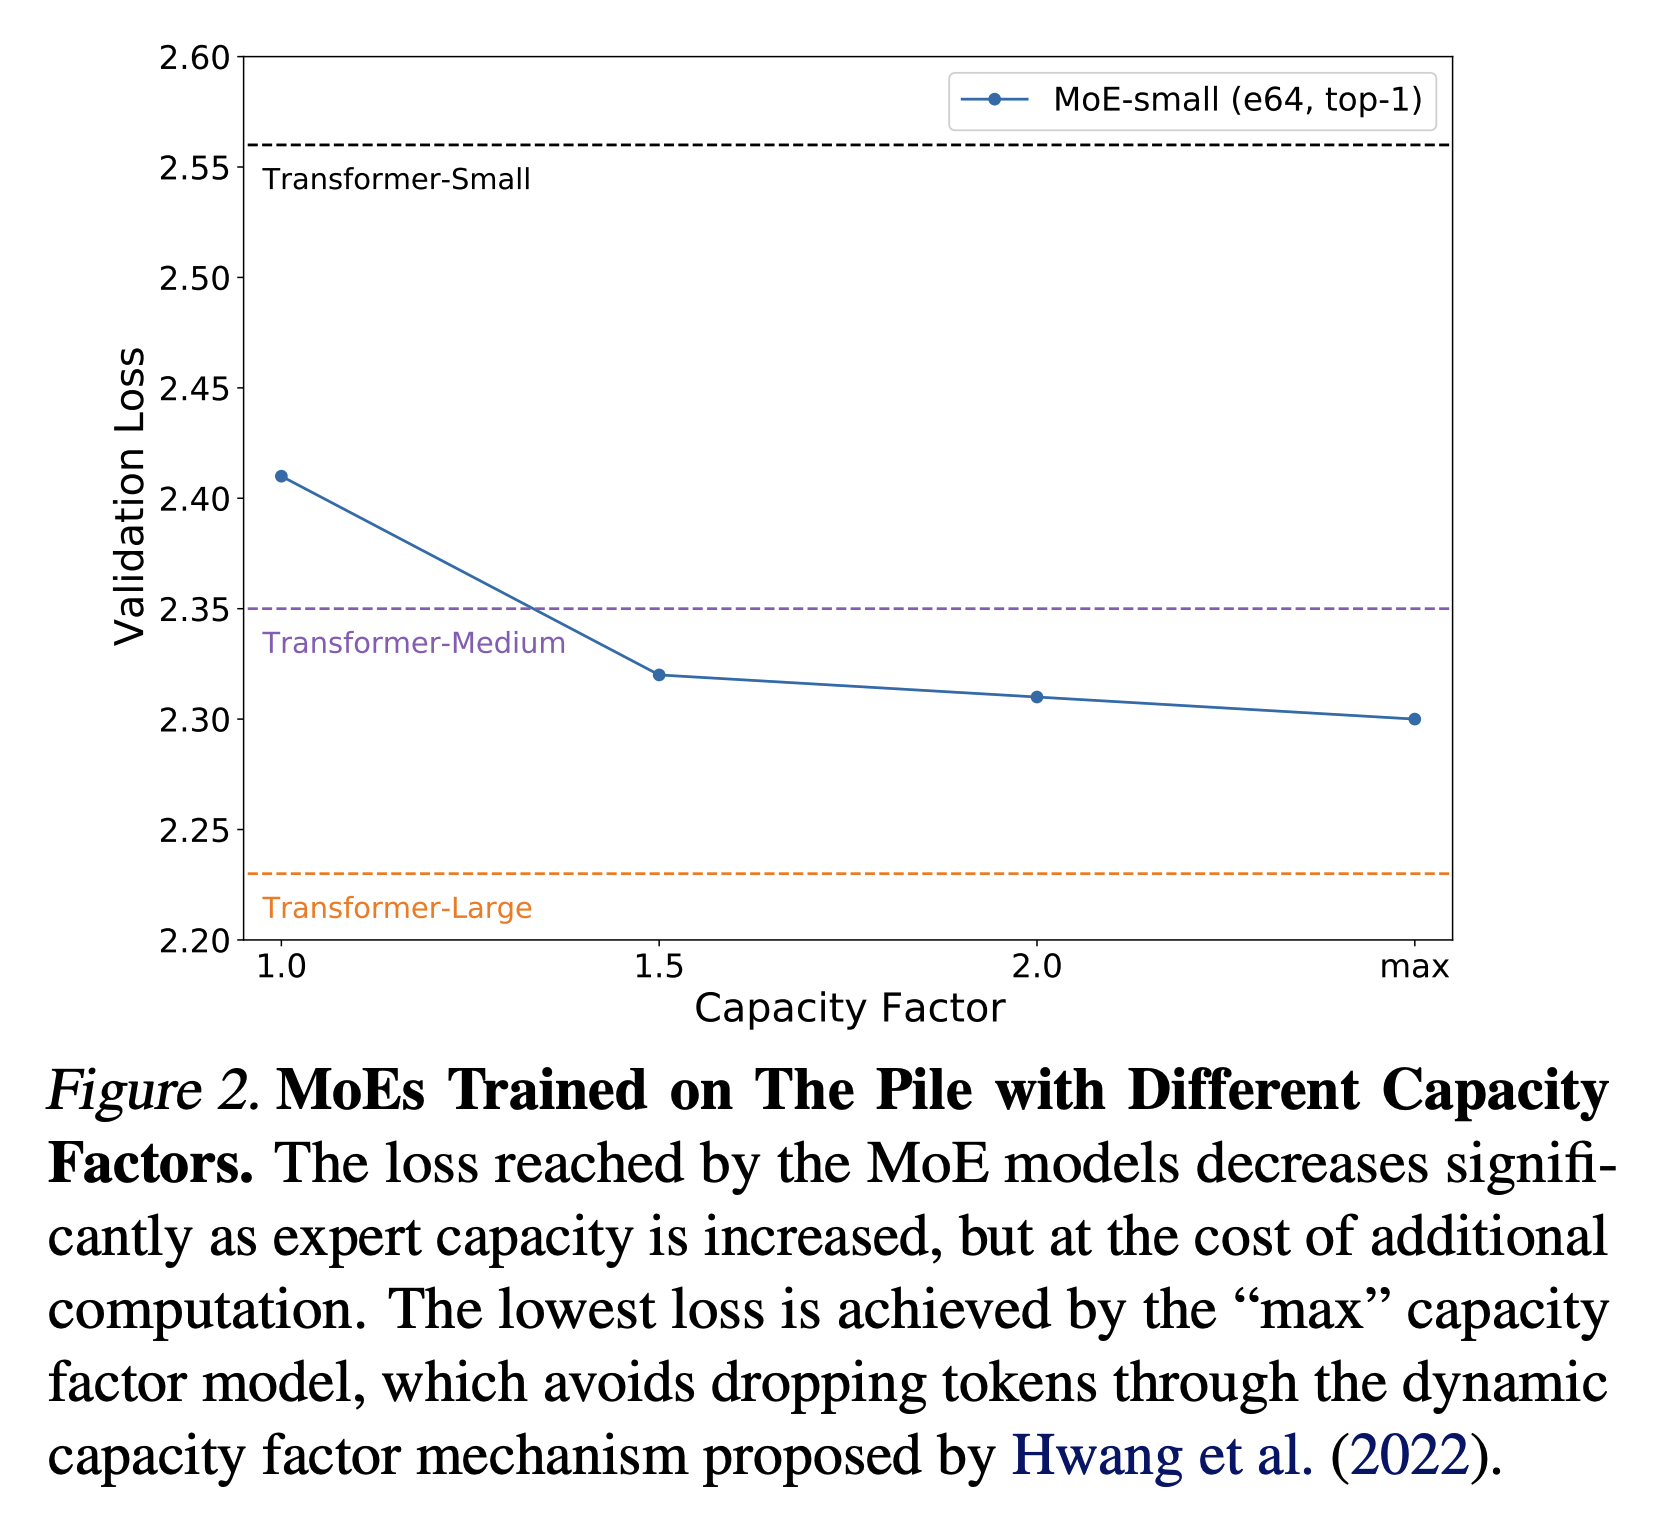
\includegraphics[width=0.95\textwidth]{images/capacity.png}
        
        \tiny Figure: Effect of capacity factor on model quality.
        \end{center}
    \end{columns}
\end{frame}

\section{Idea}
\begin{frame}{4. Idea: Block Diagonal Reformulation (1)}
    \begin{center}
    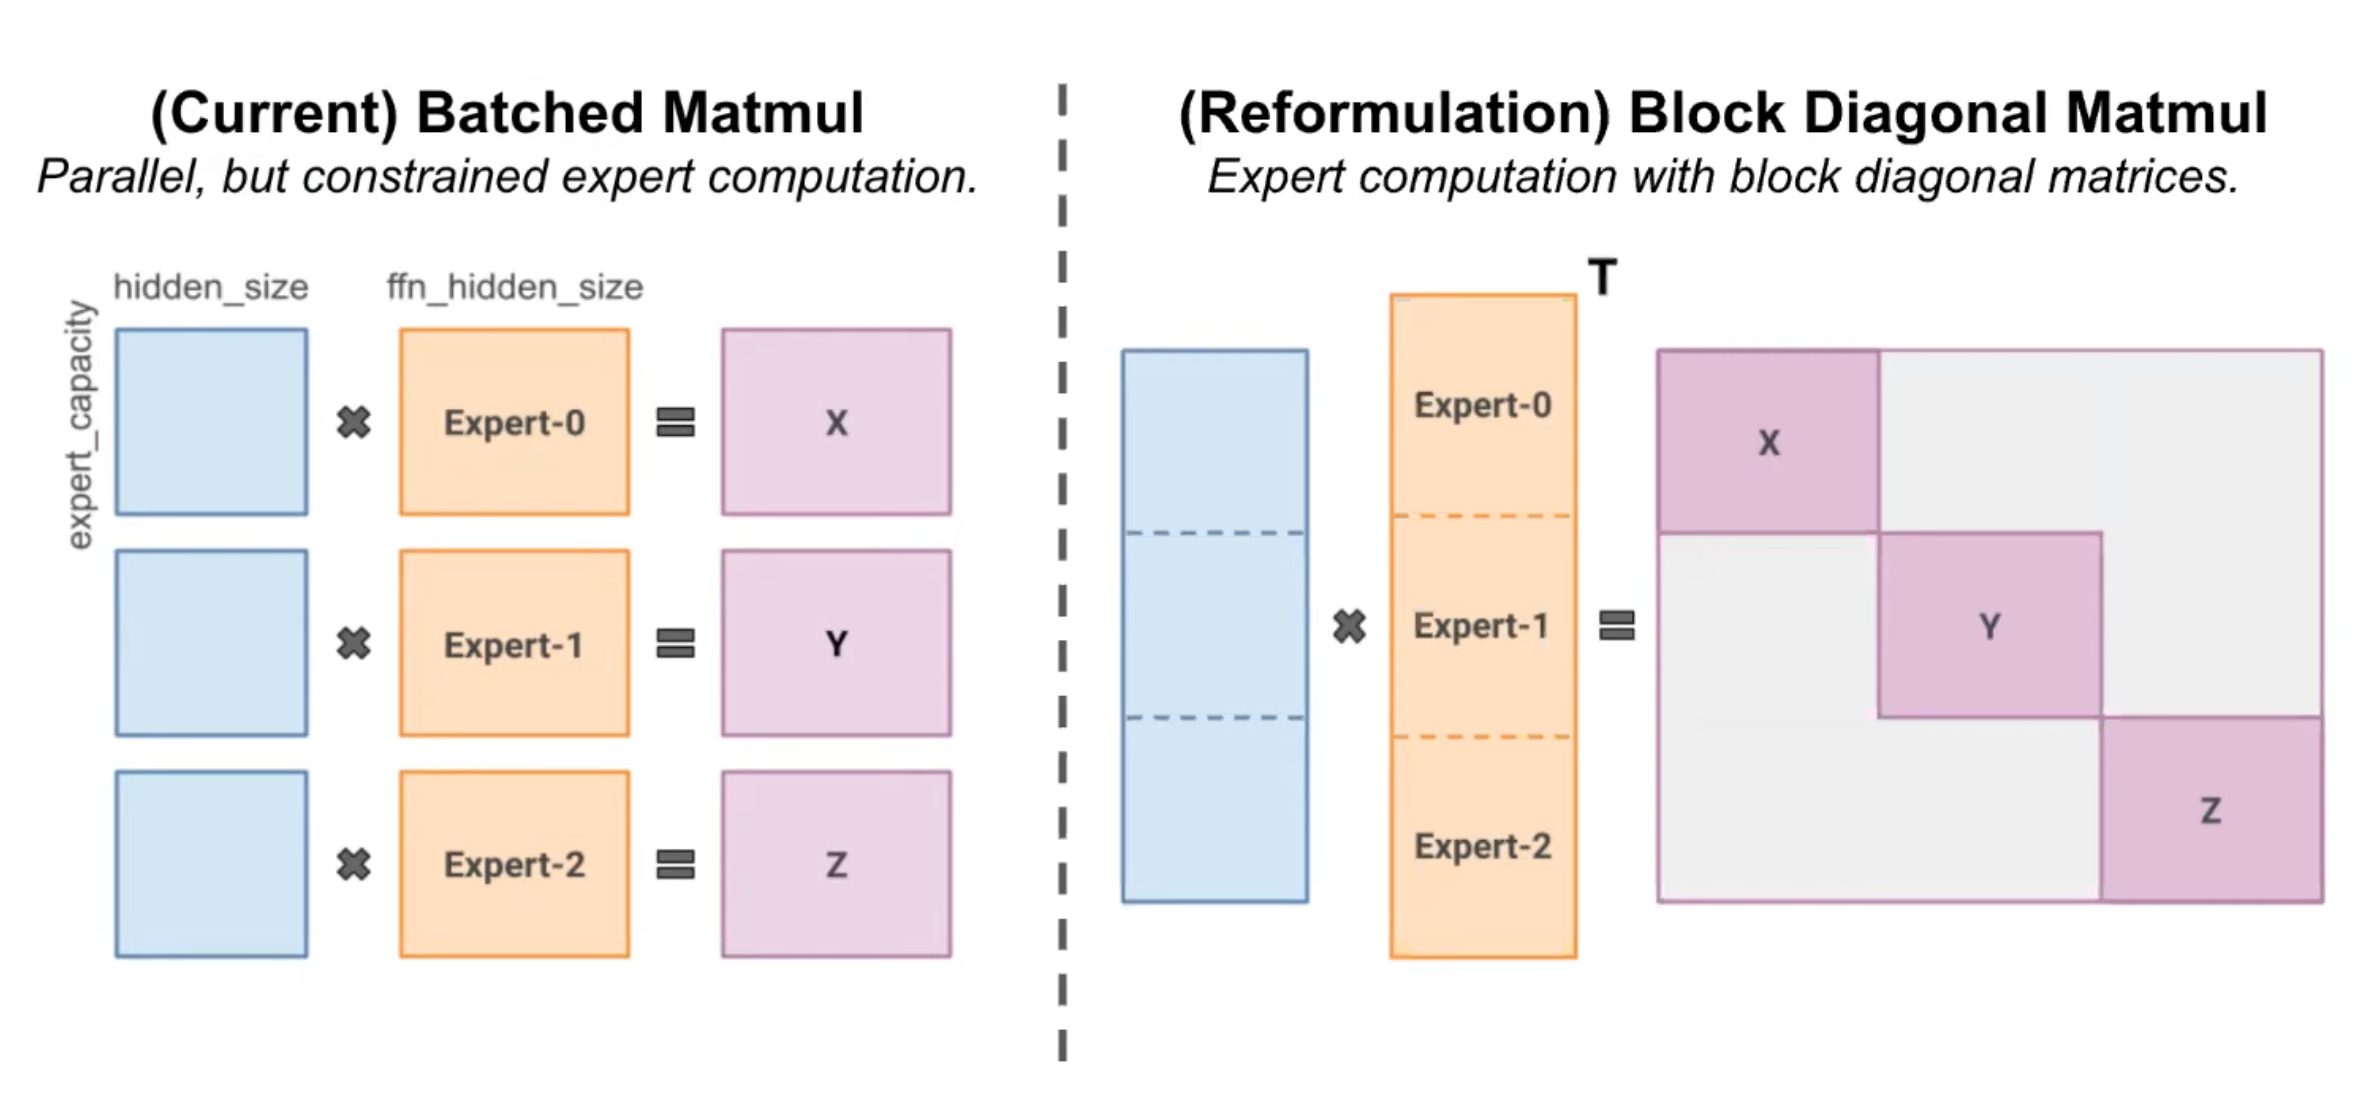
\includegraphics[width=0.85\textwidth]{images/block-diagonal.png}
    
    \medskip
    
    \footnotesize
    MegaBlocks reformulates MoE computation as block-diagonal matrix operations, \\
    enabling efficient GPU implementation without token dropping.
    \end{center}
\end{frame}

\begin{frame}{4. Idea: Block Diagonal Reformulation (2)}
    \begin{center}
    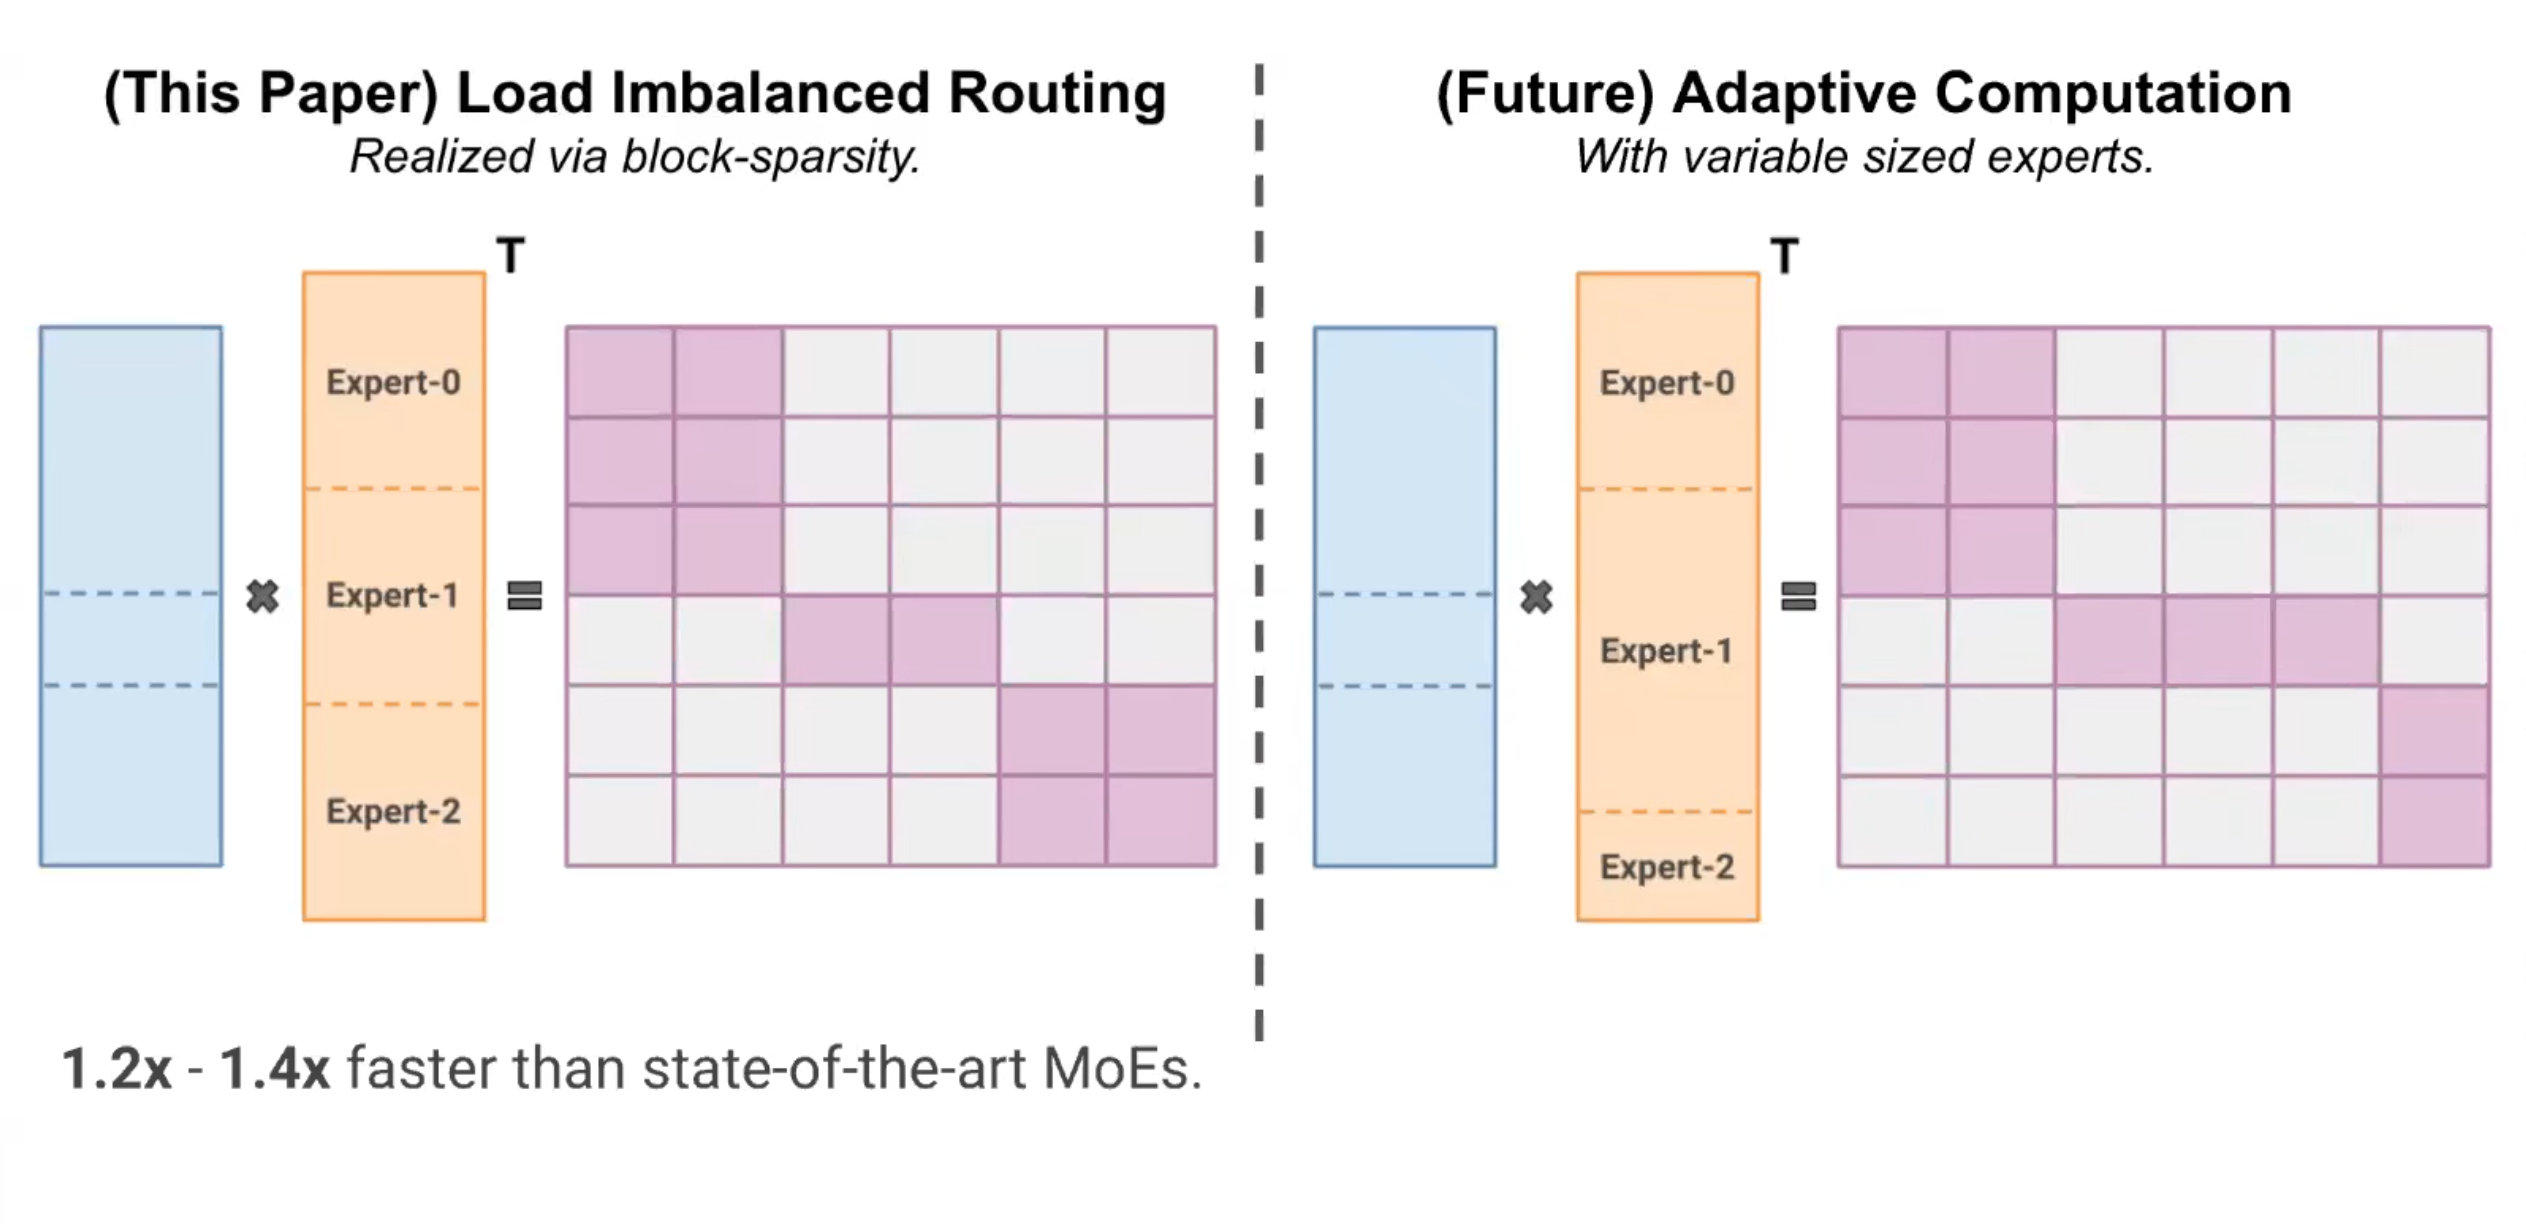
\includegraphics[width=0.85\textwidth]{images/load-imbalanced-routing.png}
    
    \medskip
    
    \footnotesize
    Handling load-imbalanced routing through block-sparse operations \\
    allows dynamic token assignment without capacity constraints.
    \end{center}
\end{frame}

\begin{frame}[shrink]{4. Recap: Sparse Matrix Product Notation}
    \begin{block}{Notation System}
    \footnotesize
    Borrowed from Triton (Tillet et al., 2019) to describe sparse/dense matrix multiplication operations
    \end{block}
    
    \begin{block}{Three-Character String Format}
    \footnotesize
    \begin{itemize}
        \item Each character is either \textbf{S} (Sparse) or \textbf{D} (Dense)
        \item Order: \textbf{Output} → \textbf{Left Input} → \textbf{Right Input}
    \end{itemize}
    \end{block}
    
    \begin{block}{Examples}
    \footnotesize
    \begin{itemize}
        \item \textbf{SDD}: Sparse output, Dense × Dense inputs
        \begin{itemize}
            \item Also known as Sampled Dense-Dense Matrix Multiplication (SDDMM)
        \end{itemize}
        \item \textbf{DSD} vs \textbf{DDS}: Different forms of Sparse Matrix-Dense Matrix Multiplication (SpMM)
        \item \textbf{SDD\textsuperscript{T}}: SDD with transposed right-hand input
    \end{itemize}
    \end{block}
\end{frame}

\begin{frame}[fragile]{4. dMoE (dropless MoE) Forward Pass Pseudocode}
    \begin{block}{MegaBlocks dMoE Implementation}
    \lstset{style=pythonstyle}
    \begin{lstlisting}
# x.shape: (num_tokens, hidden_size)
def dmoe_forward(self, x):
    # (1) Assign tokens to experts.
    # indices.shape: (num_tokens)
    # weights.shape: (num_tokens)
    indices, weights = router(x)

    # (2) Create the sparse matrix topology.
    # This describes the matrix in Figure of Block Diagonal Reformulation slide.
    topology = make_topology(indices)

    # (3) Permute the tokens to group by expert.
    x = padded_gather(x, indices)

    # (4): Compute the expert layers.
    # inner_dim = ffn_hidden_size * num_experts
    # self.w1.shape: (hidden_size, inner_dim)
    # self.w1.shape: (inner_dim, hidden_size)
    x = sdd(x, self.w1, topology)
    x = dsd(x, self.w2)

    # (5) Un-permute the tokens and scale.
    x = padded_scatter(x, indices)
    return x * weights
    \end{lstlisting}
    \end{block}
\end{frame}

\begin{frame}[fragile]{4. dMoE (dropless MoE) Expert Computation}
    \begin{block}{Expert Layer Computation Details}
    \footnotesize
    \begin{itemize}
        \item SDD (Sparse-Dense-Dense) operation for the first layer: $x = \text{SDD}(x, W_1, \text{topology})$
        \item DSD (Dense-Sparse-Dense) operation for the second layer: $x = \text{DSD}(x, W_2)$
    \end{itemize}
    \end{block}
    
    \begin{center}
    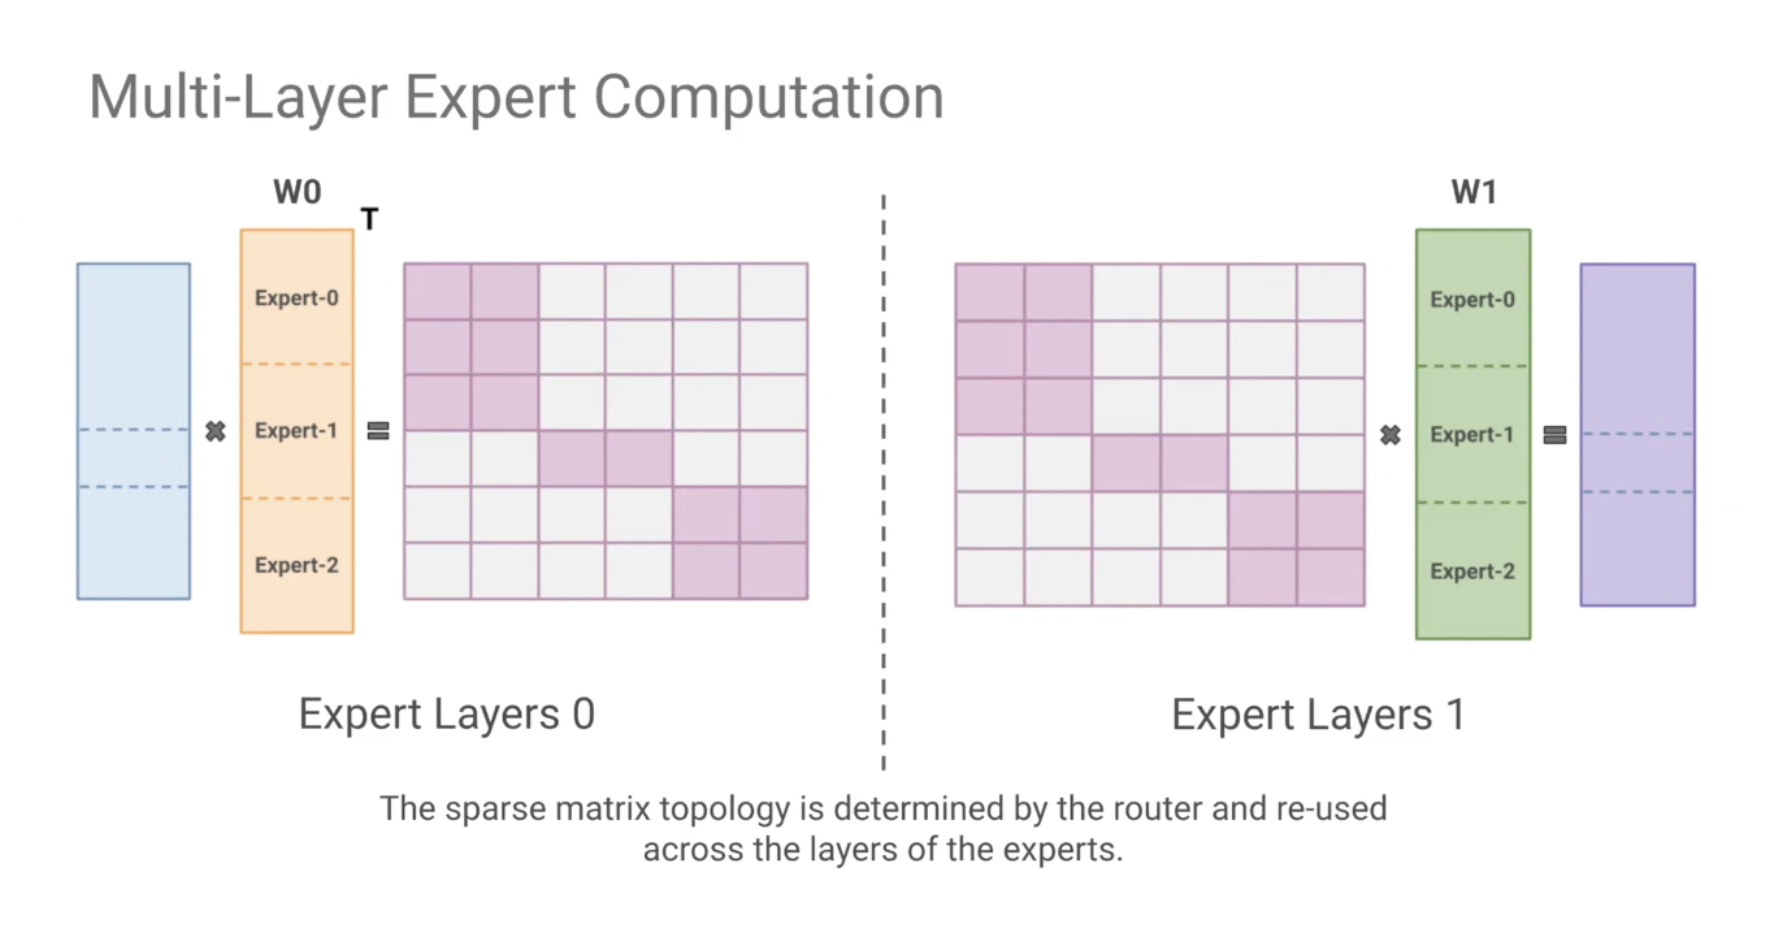
\includegraphics[width=0.75\textwidth]{images/expert_computation.png}
    
    \tiny Figure: Expert computation in dMoE using block-sparse operations.
    \end{center}
\end{frame}

\begin{frame}[fragile]{4. Efficient Block-Sparse Kernels for MoEs}
    
    \begin{columns}[t]
    \begin{column}{0.48\textwidth}
        \begin{block}{Forward Pass}
        \footnotesize
        \begin{itemize}
            \item First layer: \textbf{SDD}
            \item Second layer: \textbf{DSD}
        \end{itemize}
        \end{block}
    \end{column}
    
    \begin{column}{0.48\textwidth}
        \begin{block}{Backward Pass}
        \footnotesize
        \textbf{Second Layer:}
        \begin{itemize}
            \item Data gradient: $\text{SDD}^T$
            \item Weight gradient: $\text{DS}^T\text{D}$
        \end{itemize}
        \textbf{First Layer:}
        \begin{itemize}
            \item Data gradient: $\text{DSD}^T$
            \item Weight gradient: $\text{DD}^T\text{S}$
        \end{itemize}
        \end{block}
    \end{column}
    \end{columns}
\end{frame}

\begin{frame}{4. Tile Size Selection Experiments}

    \begin{center}
    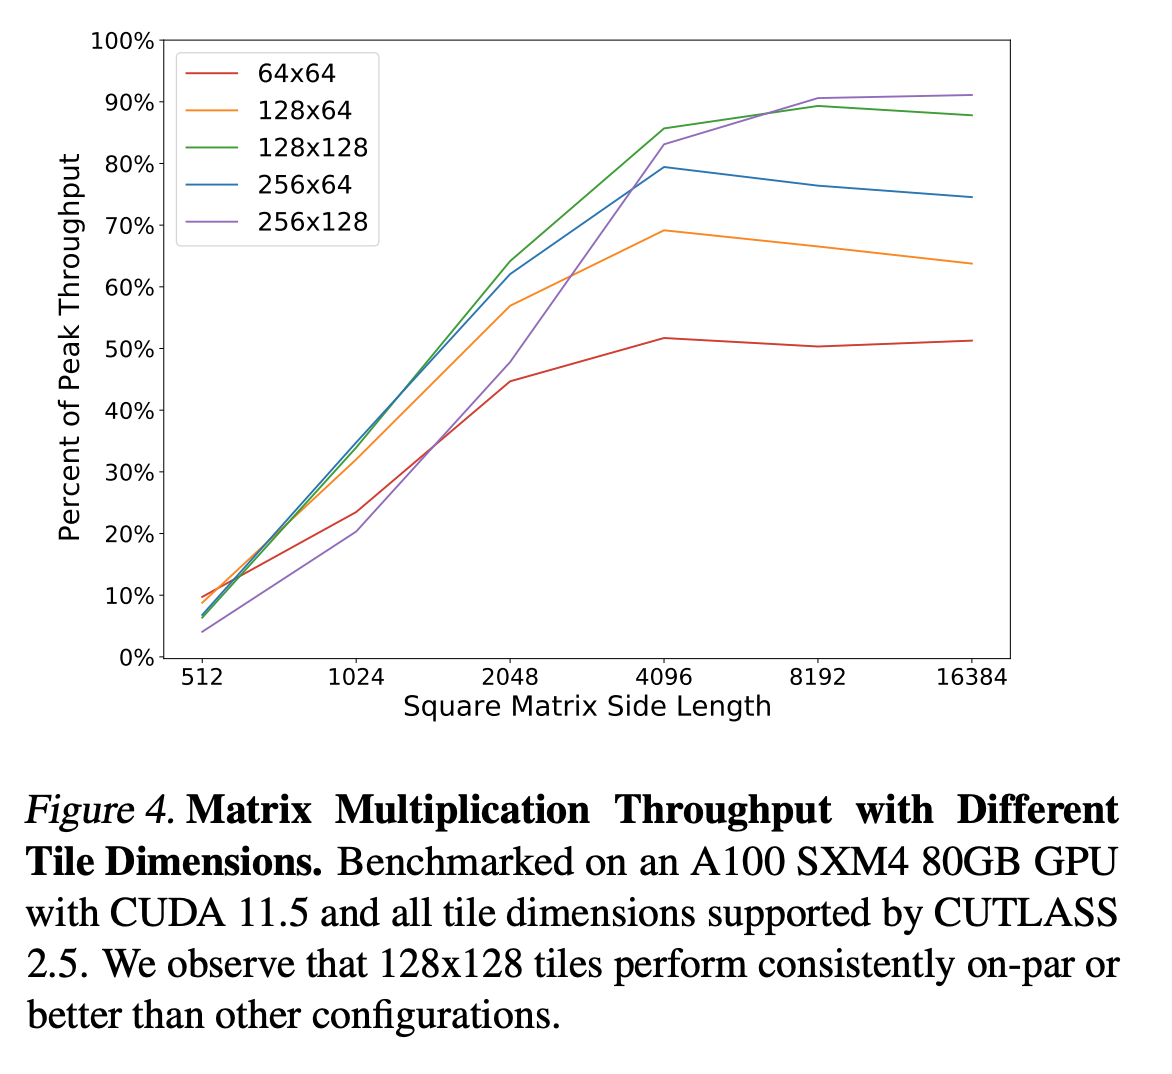
\includegraphics[width=0.6\textwidth]{images/moe_figure4.png}
    
    \tiny Figure: Performance comparison across different tile sizes. Optimal tile size balances computational efficiency and memory overhead.
    \end{center}
\end{frame}

\begin{frame}{4. MegaBlocks Approach}
    \begin{block}{One Liner Summary}
    Reformulate MoE computation in terms of \textbf{block-sparse operations}
    \end{block}
    
    \begin{block}{New Block-Sparse GPU Kernels}
    Efficiently handle the dynamism present in MoEs
    \end{block}
    
    \begin{block}{Benefits}
    \begin{itemize}
        \item Never drops tokens
        \item Maps efficiently to modern hardware
        \item Enables significant speedups
    \end{itemize}
    \end{block}
\end{frame}

\section{Implementation Details}

\begin{frame}{5. Block-Sparse Kernels for MoEs}

\centering
\vspace{0.5cm}

\renewcommand{\arraystretch}{1.4}
\setlength{\tabcolsep}{10pt}

\begin{tabular}{|l|c|c|}
\hline
\textbf{Feature} & \textbf{cuSPARSE} & \textbf{Triton Blocksparse} \\
\hline
\textbf{Large Blocks} & {\Large \checkmark} & {\Large \checkmark} \\
\hline
\textbf{Transposition} & {\Large \textcolor{red}{$\times$}} & {\Large \checkmark} \\
\hline
\textbf{Load Imbalance} & {\Large \textcolor{red}{$\times$}} & {\Large \checkmark} \\
\hline
\textbf{Fast Construction} & {\Large \textcolor{red}{$\times$}} & {\Large \textcolor{red}{$\times$}} \\
\hline
\end{tabular}


\end{frame}

\begin{frame}{5. Why These Features Matter}
    \begin{block}{Large Blocks}
    For \textbf{high throughput}: larger blocks enable better GPU utilization and performance
    \end{block}
    
    \begin{block}{Transposition}
    For \textbf{backward pass}: transpose operations are essential for efficient gradient computation
    \end{block}
    
    \begin{block}{Load Imbalance}
    \textbf{Load imbalance}: each expert processes different token counts. \\
    For \textbf{no token dropping}: must handle unbalanced expert assignments.
    \end{block}
    
    \begin{block}{Fast Construction}
    For \textbf{changes every use}: sparse pattern changes dynamically per forward/backward pass
    \end{block}
\end{frame}

\begin{frame}{5. Key Issues with Existing Libraries}
    \begin{alertblock}{cuSPARSE Limitations}
    \begin{itemize}
        \item No transpose support
        \item ELLPACK format not suitable for dynamic patterns
        \begin{itemize}
            \scriptsize
            \item ELLPACK: fixed-width sparse format assuming uniform row length
            \item Cannot efficiently handle varying expert assignment patterns
        \end{itemize}
        \item \textbf{Not an option for MoE training}
    \end{itemize}
    \end{alertblock}
    
    \begin{alertblock}{Triton Blocksparse Limitations}
    \begin{itemize}
        \item Expensive preprocessing required
        \item \textbf{5--10x slower than dense if not amortized}
        \begin{itemize}
            \scriptsize
            \item Amortized: spreading preprocessing cost over many uses
            \item MoE routing changes every iteration, so no amortization possible
        \end{itemize}
        \item Cannot reconstruct pattern efficiently every iteration
    \end{itemize}
    \end{alertblock}
\end{frame}

\begin{frame}[fragile]{5. Their Solution: Hybrid Block Sparse Format}
    \begin{block}{Kernel Design for Block-Sparse Operations}
    \scriptsize
    Extended NVIDIA's CUTLASS GEMM framework to directly handle block-sparse matrices.
    \end{block}
    
    \begin{columns}[t]
    \begin{column}{0.48\textwidth}
        \begin{block}{Hybrid BCSR-COO}
        \scriptsize
        \textbf{BCSR:} Blocked Compressed Sparse Row \\
        \textbf{BCOO:} Blocked Coordinate Format
        
        \vspace{0.1cm}
        \textbf{Problem:} SDD needs output block coordinates upfront.
        
        \textbf{Solution:} Materialize row indices
        \begin{itemize}
            \scriptsize
            \item O(1) coordinate lookup
            \item ~0.024\% overhead (128×128)
            \item Maintains row-order access
        \end{itemize}
        \end{block}
    \end{column}
    
    \begin{column}{0.48\textwidth}
        \begin{block}{Transpose Indices}
        \scriptsize
        \textbf{Problem:} Transpose access expensive in BCSR.
        
        \textbf{Solution:} Index array (no value copy)
        \begin{itemize}
            \scriptsize
            \item Points to offset in value array
            \item Indirect transposed access
            \item Minimal memory overhead
        \end{itemize}
        \end{block}
    \end{column}
    \end{columns}
\end{frame}

\begin{frame}{5. Hybrid Block Sparse Format Illustration}
    \begin{center}
    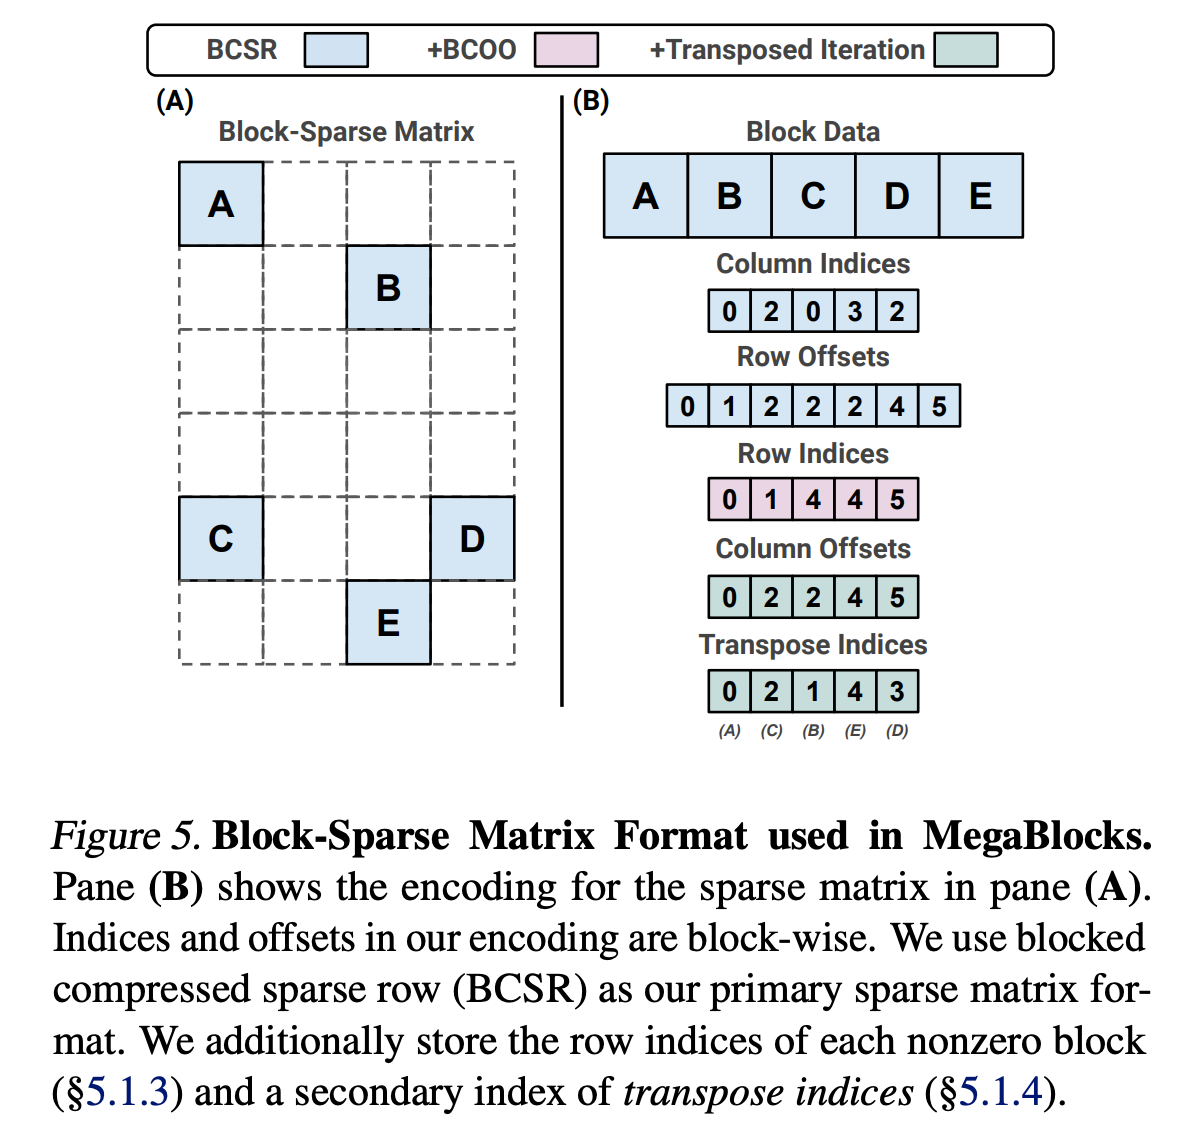
\includegraphics[width=0.65\textwidth]{images/moe_figure5.png}
    \end{center}
    \vspace{-0.2cm}
    \tiny Figure: Hybrid blocked-CSR-COO format with transpose indices.
\end{frame}

\section{Experimental Results}

\begin{frame}{6. Experimental Evaluation}
    \begin{block}{Three Key Experiments}
    \footnotesize
    This work evaluates MegaBlocks through three different experimental setups:
    \end{block}
    
    \vspace{0.3cm}
    
    \begin{enumerate}
        \item \textbf{MoE Training Without Dropping Tokens}
        
        \vspace{0.2cm}
        
        \item \textbf{MoE Training With Token Dropping}
        
        \vspace{0.2cm}
        
        \item \textbf{Block-Sparse Matrix Multiplication Performance}
        \begin{itemize}
            \footnotesize
            \item Benchmarking the custom block-sparse kernels
        \end{itemize}
    \end{enumerate}
\end{frame}


\begin{frame}{6. Evaluation}
    \begin{block}{Implementation}
    \scriptsize
    MegaBlocks is built on Megatron-LM + PyTorch.
    \end{block}
    
    \begin{block}{Models}
    \scriptsize
    Transformers-MoEs with 64-experts and top-1 routing.
    \end{block}
    
    \begin{block}{Baselines}
    \scriptsize
    \textbf{MoE:} Tutel (+ Megatron-LM) \\
    \textbf{Dense:} Megatron-LM
    \end{block}
    
    \begin{block}{Training}
    \scriptsize
    10B tokens from The Pile on 8x A100 GPUs. \\
    Data parallelism for Transformers, 8-way expert model parallelism for MoE layers. \\
    capacity\_factor=\{1, 1.5, 2.0\} for MoE baselines.
    \end{block}
\end{frame}

\begin{frame}{6. Model Configurations}
    \begin{table}
    \scriptsize
    \centering
    \caption{Baseline Transformer Models}
    \vspace{-0.1cm}
    \begin{tabular}{lcccc}
    \hline
    \textbf{Model} & \textbf{h\_size} & \textbf{layers} & \textbf{Weights(M)} & \textbf{GFLOPs} \\
    \hline
    XS & 512 & 6 & 46 & 316 \\
    Small & 768 & 12 & 125 & 879 \\
    Medium & 1024 & 24 & 356 & 2487 \\
    Large & 1536 & 24 & 760 & 5122 \\
    XL & 2048 & 24 & 1316 & 8684 \\
    \hline
    \end{tabular}
    \end{table}
    
    \vspace{0.3cm}
    
    \begin{table}
    \scriptsize
    \centering
    \caption{Transformer-MoE Models}
    \vspace{-0.1cm}
    \begin{tabular}{lcccc}
    \hline
    \textbf{MoE} & \textbf{num\_exp} & \textbf{top\_k} & \textbf{Weights(M)} & \textbf{GFLOPs} \\
    \hline
    XS & 64 & 1 & 839 & 316 \\
    Small & 64 & 1 & 3,693 & 879 \\
    Medium & 64 & 1 & 13,041 & 2487 \\
    \hline
    \end{tabular}
    \end{table}
\end{frame}

\begin{frame}{6. Experiment 1: MoE Training Without Dropping Tokens}
    \begin{center}
    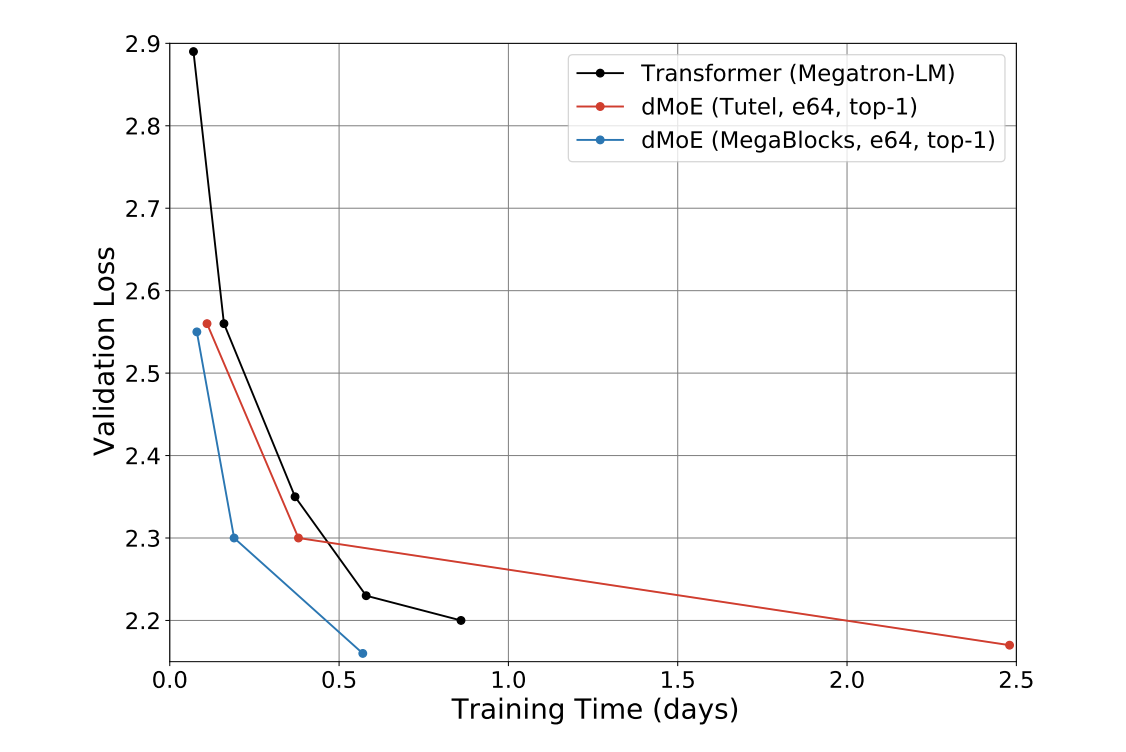
\includegraphics[width=0.80\textwidth]{images/moe_figure7.png}
    \end{center}
    \vspace{-0.2cm}
    \tiny Figure 7: Performance comparison of dropless MoE training with MegaBlocks.
\end{frame}

\begin{frame}{6. Experiment 2: MoE Training With Token Dropping}
    \begin{center}
    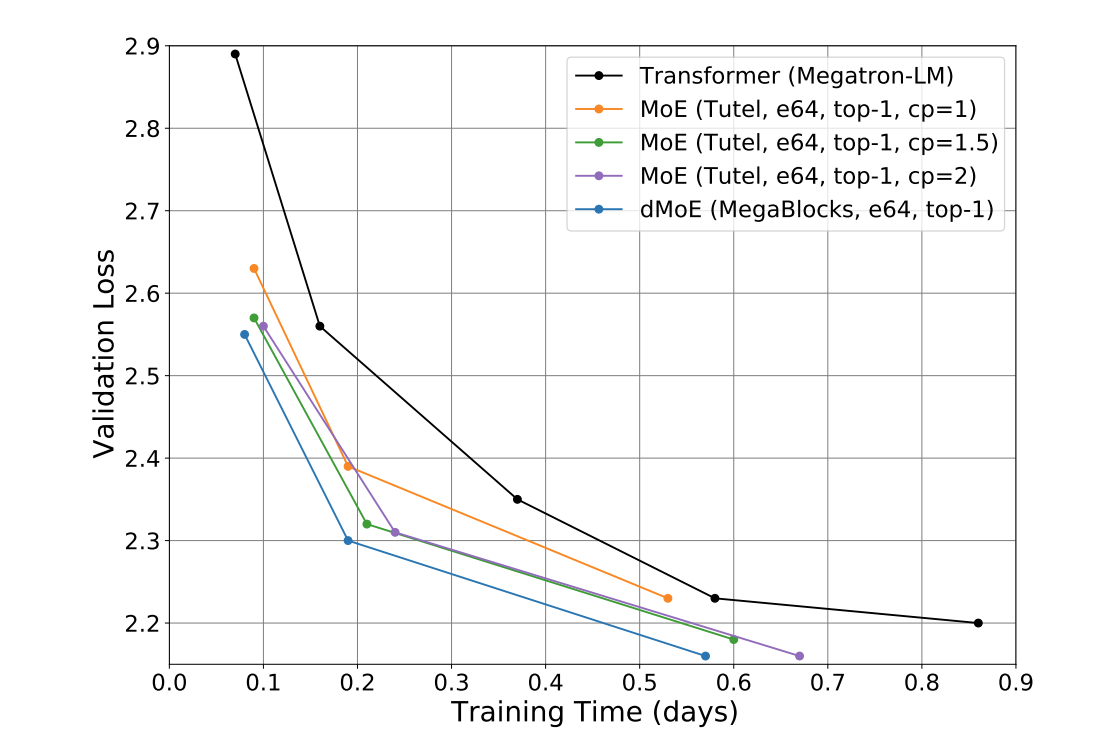
\includegraphics[width=0.80\textwidth]{images/moe_figure8.png}
    \end{center}
    \vspace{-0.2cm}
    \tiny Figure 8: Comparison with traditional token-dropping approaches.
\end{frame}

\begin{frame}{6. Experiment 3: Block-Sparse Matrix Multiplication Performance}
    \begin{center}
    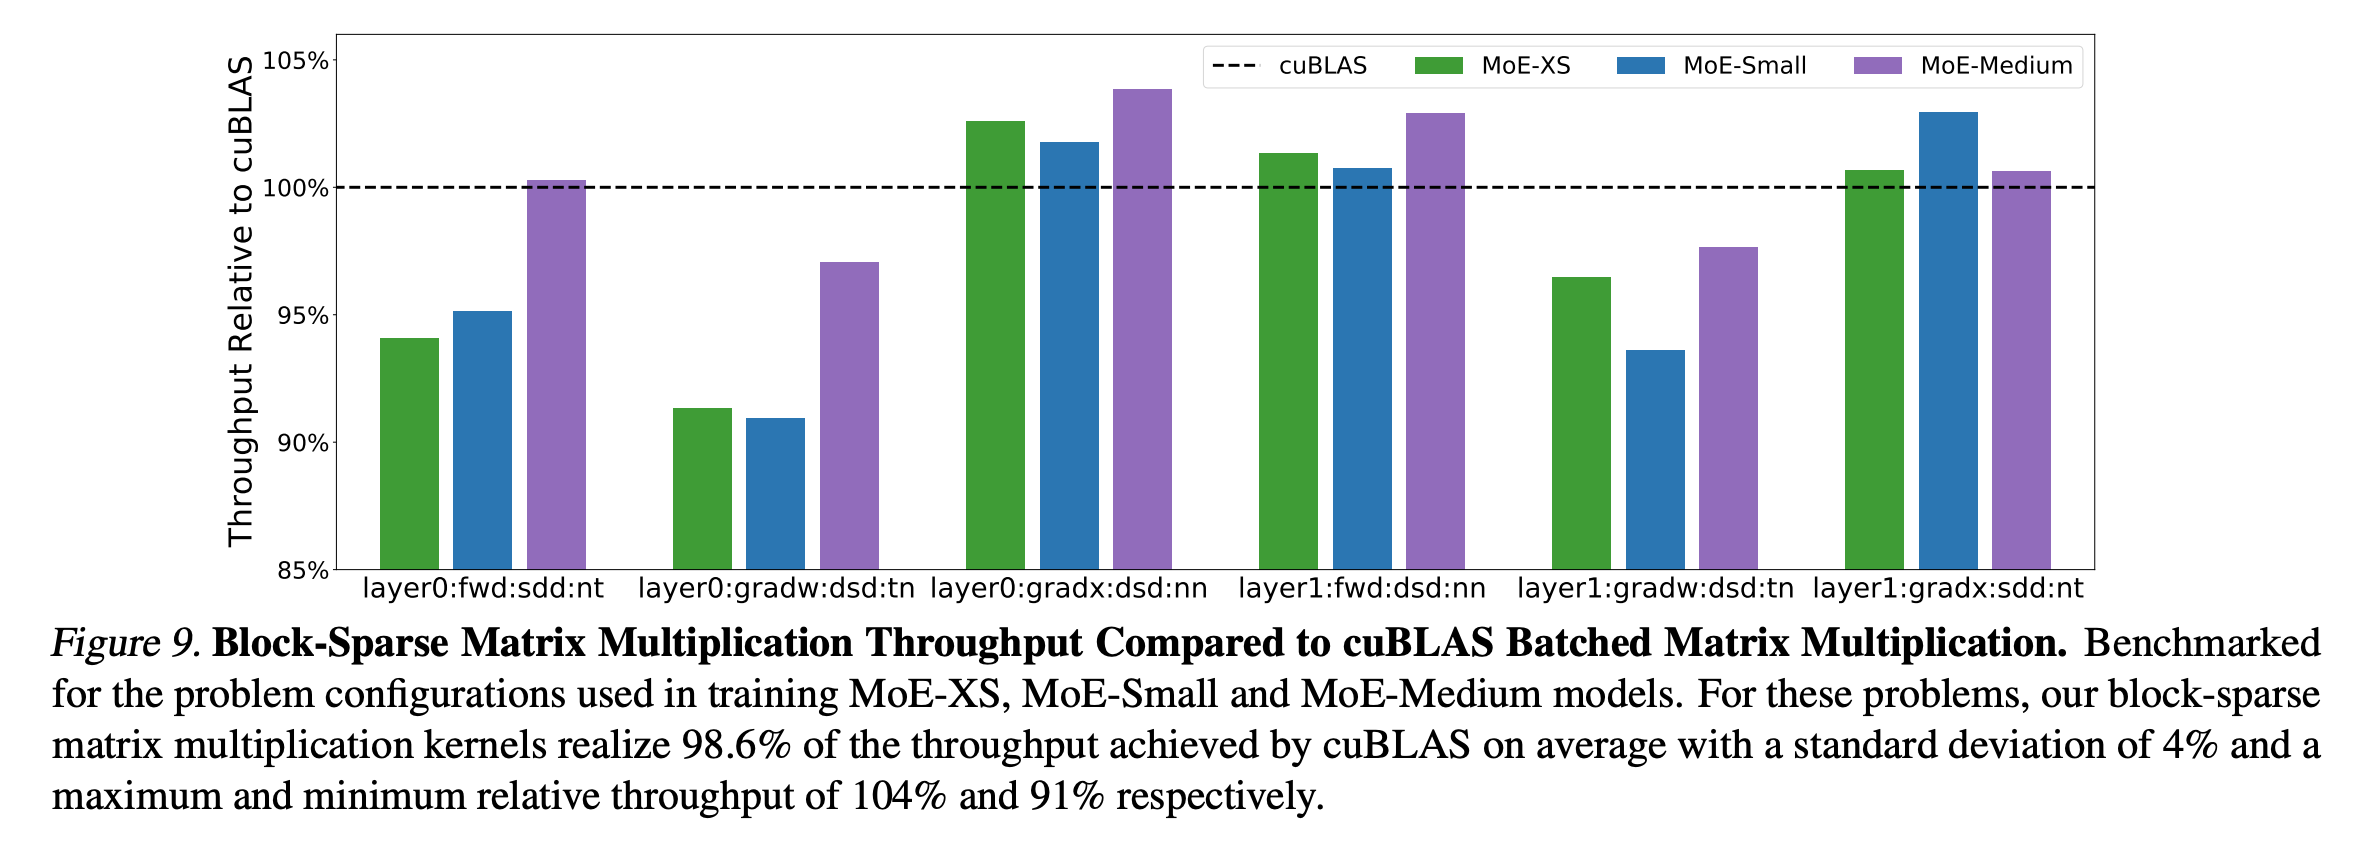
\includegraphics[width=0.90\textwidth]{images/moe_figure9.png}
    \end{center}
    \vspace{-0.3cm}
    \tiny Figure 9: Microbenchmark results of custom block-sparse kernels.
    
    \vspace{0.2cm}
    
    \begin{alertblock}{Observed Overhead in Weight Gradients}
    \scriptsize
    \textbf{DSTD operation} (weight gradient with transposed sparse operand) shows overhead:
    \begin{itemize}
        \scriptsize
        \item Uses \textbf{secondary index} for transpose access (no value copy/transpose)
        \item Weak spatial locality → reduced cache utilization → lower throughput

    \end{itemize}
    \end{alertblock}
\end{frame}

\section{Discussion}
\begin{frame}{7. Discussion Question}
    \begin{block}{Hardware Trend vs. MoE Direction}
    MoE models use less computation relative to their model size. \\
    However, on modern GPUs, computation is becoming relatively cheap while memory is increasingly expensive.
    \end{block}
    
    \begin{alertblock}{Key Question}
    This seems opposite to hardware trends—does this direction still make sense?
    \end{alertblock}
    
\end{frame}

\section{Additional References}
\begin{frame}[allowframebreaks]{Additional References}
    \bibliography{references}
\end{frame}

\begin{frame}

\begin{center}
    Thank you!
    
    \email
\end{center}


\end{frame}

\end{document}